\documentclass[preprint, floatfix, pra, showpacs, showkeys]{revtex4}
\usepackage{graphicx}
\usepackage{dcolumn}

\newcommand{\threej}[6]{\ensuremath{\left({#1\atop #4}{#2\atop #5}
{#3\atop #6}\right)}}
\newcommand{\sixj}[6]{\ensuremath{\left\{{#1\atop #4}{#2\atop #5}
{#3\atop #6}\right\}}}

\begin{document}

\title{The Flexible Atomic Code: V. Electron Impact Ionization}  
\author{Ming Feng Gu}
\affiliation{Center for Space Research, Massachusetts Institute of Technology,
Cambridge, MA 02139} 
\email[Email: ]{mfgu@space.mit.edu}

\begin{abstract} 
The detailed level-to-level electron impact ionization cross sections are
calculated in the relativistic distorted-wave (DW) approximation, extending
the factorization-interpolation method developed for the calculation of
electron impact excitation cross sections. The implementation allows for the
most general configuration mixing to be included. Much more efficient methods
based on the Coulomb-Born-Exchange (CBE) approximation or the
Binary-Encounter-Dipole (BED) theory 
are also implemented. The present DW and CBE results for the ionization of
$2s$ and $2p$ electrons from the ground state of Ne-like iron agree with
previous non-relativistic and relativistic DW calculations to within
10-20\%. The BED cross sections are substantially smaller at low energies due
to a scaling factor delibrately introduced into the theory.
\end{abstract}

\pacs{34.80.Kw}
\keywords{Distorted-wave; Electron impact ionization}
\maketitle

\section{Introduction}
This is the fifth paper of a sequence describing a systematic software
package, the Flexible Atomic Code (FAC), 
for calculating atomic radiative and collisional processes in the relativistic
distorted-wave (DW) approximation. In the previous papers
\cite{gu02a,gu02b,gu02c,gu02d}, the
calculation of atomic structure, electron impact excitation (EIE),
non-resonant photoionization and radiative recombination, autoionization and
dielectronic recombination are discussed. This paper deals with the direct
ionization by electron impact (EII). Accurate EII cross sections are needed
to calculate the ionization balance in the modeling of hot plasmas. Inner
shell EII is also important as an emission line formation process. 

Several DW programs have been developed for the calculation of EII cross
sections in the past decades, in either non-relativistic \cite{younger80} or
relativistic \cite{pindzola88, sampson91} approximations. The present program
is similar to that of \textcite{sampson91} in particular,  which extends the
efficient factorization-interpolation method of \textcite{barshalom88} to the
calculation of EII cross sections, and leads to great simplifications for
complex ions. The essence of the factorization method is the separation of
the angular and radial parts in the formula of EII cross sections. The angular
part depends on the angular momentum coupling of the target states, while the
radial part only depends on the one-electron radial orbitals, without
explicit reference to the initial and final states involved in the
process. Different initial and final states affect the radial part only
implicitly through the ionization energy due to the energy conservation. Such
a separation enables the rapid calculation of the radial integrals on a few
ionization energy points, the integrals at actual ionization energies are
obtained by interpolation.  

The present program also implements much more efficient methods based on the
Coulomb-Born-Echange approximation (CBE) or the Binary-Encounter-Dipole (BED)
theory of \textcite{kim94}. The CBE implementation makes use of the
parametrized reduced cross sections of \textcite{golden77, golden80}, and the
BED implementation uses the bound-free differential oscillator strengths
calculated by the present program \cite{gu02c}. The CBE results are close to
the non-relativistic DW cross sections, while the BED cross sections are
substantially smaller at low energies due to a scaling factor deliberately
introduced into the theory, which appear to improve the agreements with
experimental results in many cases \cite{kim94}.
 
Section \ref{sec_theory} presents a brief theoretical background and some
important numerical techniques used in the program. Section \ref{sec_results}
illustrates the correctness of the present program by calculating the
ionization cross sections of Ne-like iron, and comparing the results to the
previous publications. Section \ref{sec_conclusions} gives a brief summary.

\section{Theory and Numerical Techniques}
\label{sec_theory}
\subsection{Relativistic Distorted-wave Theory}
The formula for EII cross section, differential in energy of the ejected
electron, may be obtained from that for EIE by replacing one bound orbital in
the final state with the free orbital of the ejected electron and summing 
over its angular momentum. It can be expressed in terms of the collision
strength similar to that of EIE 
\begin{equation}
\label{eq_cross}
\sigma(\varepsilon_0,\varepsilon) = \frac{1}{k_0^2g_0}\Omega_{01},
\end{equation}
where $\varepsilon_0$ and $k_0$ are the energy and kinetic momentum of the
incident electron, $\varepsilon$ is the energy of the ejected electron. The
normalization of continuum orbitals is discussed in Ref.~\cite{gu02b}. Note
that the absence of the 
factor $\pi$ as compared with the formula for the EIE cross section is due to
the different normalization of the free and bound orbitals. The collision
strength $\Omega_{01}$ is \cite{gu02b}
\begin{equation}
\label{eq_cs}
\Omega_{01} = 2\sum_{\kappa,J_T\atop k,\alpha_0\beta_0}
Q^k(\alpha_0\kappa;\beta_0\kappa)
<\psi_0||Z^k(\alpha_0,\kappa)||\psi_1,\kappa;J_T>
<\psi_0||Z^k(\beta_0,\kappa)||\psi_1,\kappa;J_T>,
\end{equation}
where $\kappa$ is the relativistic angular quantum number of the ejected
electron, $J_T$ is the total angular momentum of the final state coupled with
the ejected electron,
the radial part $Q^k$ is identical to that for EIE, except that one of
the bound orbitals in the final state is now replaced by a free orbital. Note
that $Q^k$ contains the summation over the partial waves of incident and
scattered electrons.

As for photoionization \cite{gu02b}, the angular factors involving the free
electron can be simplified using the decoupling formula of Racah
\begin{eqnarray}
&<&\psi_0||Z^k(\alpha_0, \kappa)||\psi_1,\kappa;J_T>
<\psi_0||Z^k(\beta_0, \kappa)||\psi_1,\kappa;J_T> = \nonumber\\*
&<&\psi_1||\tilde{a}_{\tilde{\alpha_0}}||\psi_0>
<\psi_1||\tilde{a}_{\tilde{\beta_0}}||\psi_0>
\sum_{J_T}[J_T]\sixj{J_1}{j}{J_T}{k}{J_0}{j_{\alpha_0}}
\sixj{J_1}{j}{J_T}{k}{J_0}{j_{\beta_0}},
\end{eqnarray}
where $[J_T]$ denotes $2J_T+1$ and $\sixj{j_1}{j_2}{j_3}{j_4}{j_5}{j_6}$ is
the Wigner $6j$ symbol. 
Substituting this into Eq.~(\ref{eq_cs}), and carrying
out the summation over $J_T$ analytically, we find
\begin{equation}
\label{eq_scs}
\Omega_{01} = 2\sum_{k,\alpha_0\beta_0}
\delta_{j_{\alpha_0}j_{\beta_0}}[j_{\alpha_0}]^{-1} 
\overline{Q}^k(\alpha_0,\beta_0)
<\psi_1||\tilde{a}_{\tilde{\alpha_0}}||\psi_0>
<\psi_1||\tilde{a}_{\tilde{\beta_0}}||\psi_0>,
\end{equation}
where $\overline{Q}^k(\alpha_0,\beta_0) = \sum_\kappa
Q^k(\alpha_0\kappa;\beta_0\kappa)$.
Note that since only basis states with the same parity can mix, the condition
$j_{\alpha_0}=j_{\beta_0}$ implies that $l_{\alpha_0} = l_{\beta_0}$ as
well. Therefore, if the configuration interaction is limited within the same
$n$ complex, only terms with $\alpha_0 = \beta_0$ survive in the summation. 

The total ionization cross section is obtained by integrating $\Omega_{01}$
over the energy of the ejected electron, $\varepsilon$
\begin{equation}
\label{eq_total}
\sigma(\varepsilon_0) = \int\nolimits_0^{\frac{\varepsilon_0-I}{2}}
\sigma(\varepsilon_0,\varepsilon) d\varepsilon,
\end{equation}
where $I$ is the ionization energy. The ionization energy enters the
radial integral $Q^k$ implicitly, since $\varepsilon_0 =
I+\varepsilon_1+\varepsilon$, where $\varepsilon_1$ is the energy of the
scattered electron. We choose to calculate $Q^k$ as a function of $I$,
$\varepsilon_1$, and $\varepsilon$. For a given transition array, we first set
up a three dimensional grid on these three energies. The integrals $Q^k$ are 
only calculated on this grid, values for arbitrary energies are obtained by
interpolation. For a given ionization channel with
ionization energy of $I_{01}$ and the incident electron energy of
$\varepsilon_t + I_{01}$, where $\varepsilon_t$ is the sum of the energies of
the two final free electrons, the calculation of the total cross section
proceeds as 
following. The first step is the interpolation on the $I$ grid to obtain, for
each point on the $(\varepsilon_1,\varepsilon)$ grid, the values of
$\overline{Q}^k(I_{01})$ at the actual ionization energy, $I_{01}$. We then
establish another grid for the energy of the ejected electron in the range 
from 0 to $\varepsilon_t/2$ for the purpose of the numerical integration in
Eq.~(\ref{eq_total}). For each 
point on this grid, the value of $\varepsilon_1 = \varepsilon_t-\varepsilon$
is determined. A two dimensional interpolation is then performed on the array
$\overline{Q}^k(I_{01},\varepsilon_1,\varepsilon)$ to obtain the radial
integrals at these specific 
energies. Finally the integral in Eq.~(\ref{eq_total}) is evaluated to
yield the total cross section. In practice, we find such a procedure
minimizes the number of radial integrals need to be computed explicitly. The
number of grid points for the ionization energy is chosen similarly as for the
excitation energies of EIE, that is, 2 points with linear interpolation when
the ionization energies vary by less than 20\%, and 3 points with cubic spline
interpolation otherwise. The grids for the $\varepsilon_1$ and $\varepsilon$
are usually chosen to have 6 points spanning the range necessary to cover the
collision energies where the total cross sections are needed.

For each point on the three dimensional grid $(I,\varepsilon_1, \varepsilon)$,
and bound orbitals $\alpha_0$ and $\beta_0$, the evaluation of
$\overline{Q}^k(\alpha_0,\beta_0)$ involves the summation of the 
partial waves of all free electrons. The angular momentum of the ejected
electron must satisfy the triangular relation $\Delta(j_{\alpha_0}, k, j)$,
therefore, the limit on the rank $k$ in the expansion of the Coulomb
interaction restricts the number of $\kappa$ terms. Usually $k_{max} = 6$ is
large enough to ensure the convergence. A further limit on the orbital angular
momentum of 
the ejected electron may also be specified. The summation over the partial
waves of the incident and scattered electrons proceeds exactly the same way as
in the calculation of EIE cross sections, using the Coulomb-Bethe
approximation for the high partial waves in the case of allowed integrals.

\subsection{Coulomb-Born-Exchange Approximation}
The computation of radial integrals in the DW approximation is very time
consuming. In the CBE approximation implemented in the present program, only
the terms with $\alpha_0 = \beta_0$ are retained in Eq.~(\ref{eq_scs}). After
the integration over the energy of the ejected electron, a reduced radial
integral is defined as 
\begin{equation}
\label{eq_reduced}
Q_R(\alpha_0) = I_{\alpha_0}I
\sum_k\int_0^{\frac{\varepsilon_0-I}{2}}
\overline{Q}^k(\alpha_0,\alpha_0)d\varepsilon,
\end{equation}
where $I_{\alpha_0}$ is the binding energy of the orbital $\alpha_0$. It is
well known that the reduced radial integrals are not very sensitive to the
difference in the electronic structures and nuclear charges \cite{zhang90}. We
therefore use the hydrogenic values calculated under the CBE approximation
\cite{golden77, golden80}, in the place of detailed DW radial integrals. A
simple parametrized formula as given in \textcite{zhang90} is used for this
purpose. 
\begin{equation}
Q_R = A\ln(u)+D\left(1-\frac{1}{u}\right)^2+
\left(\frac{c}{u}+\frac{d}{u^2}\right)\left(1-\frac{1}{u}\right),
\end{equation}
where $u=\varepsilon_0/I$. In fact, even in the detailed DW calculations, the
computed radial integrals are fitted with this formula, fixing the coefficient
$A$ according to the correct Bethe limit. The parameters are then used to
obtain total ionization cross sections at many incident energies. It is also
possible to use the parameters given by \textcite{fontes93} instead of the CBE
values to bring the results in better agreement with the detailed DW
calculations. 

\subsection{Binary-Encounter-Dipole Theory}
The CBE approximaiton discussed above trys to capture the detail of the ionic
structure through a universal reduced radial integral. The BED theory
combines the Mott cross section and binary encouter cross section, taking into
account the high energy Bethe limit, to derive a semi-empirical formula for
the radial integrals \cite{kim94}. The computation of bound-free differential
oscillator strengths, which are related to the Bethe coefficients, is much
simpler than the DW calculation of ionization radial integrals. Therefore the
BED implementation is very efficient in practice. A unique feature of the BED
theory is the energy denominator $\varepsilon_0+I$ (for neutral atoms, the
average kinetic energy of the active bound electron should also be added), as
opposed to $\varepsilon_0$ in various first order Born approximaitions
(including DW). This modification effectively introduces a scaling factor
$\varepsilon_0/(\varepsilon_0+I)$, which reduces the ionization cross sections
at low energies. Comparison with experimental results for Low-Z near neutral
ions indicates that such scaling brings the theoretical results in better
agreement with experiments \cite{kim94}. However, for highly charged ions, we
find that this scaling reduces the cross sections by a too large factor. A
modified scaling factor is therefore introduced as
$\varepsilon_0/(\varepsilon_0+I_s)$ with
\begin{equation}
I_s = \frac{N}{2Z-N}I,
\end{equation}
where $N$ is the number of electrons of the ion and $Z$ is the atomic
number.

\begin{figure}
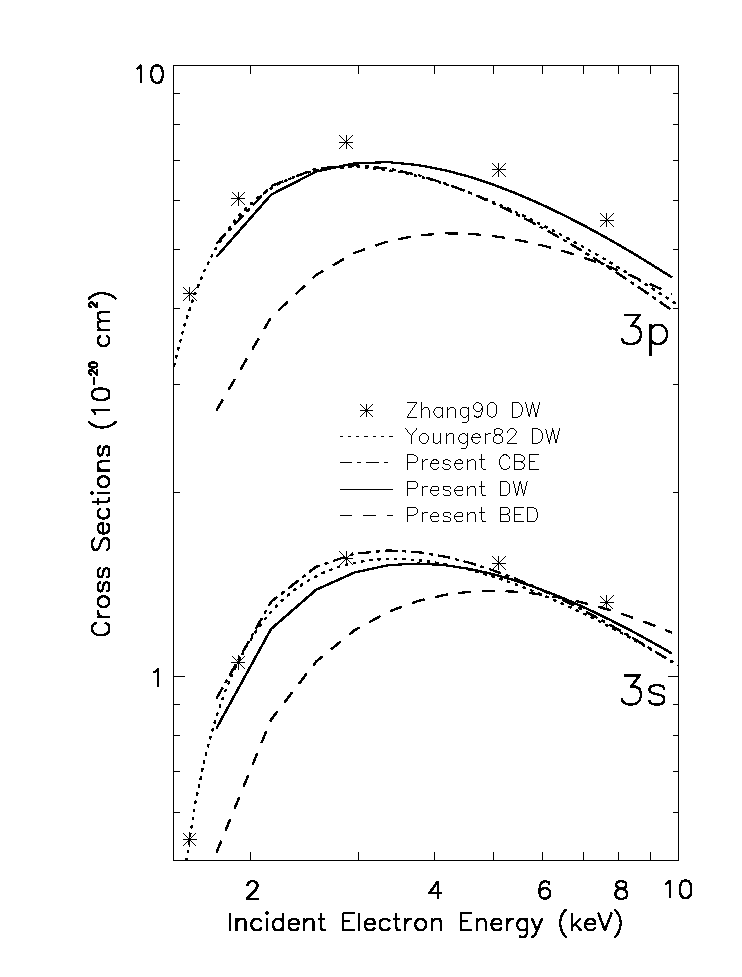
\includegraphics[width=5in]{ion.eps}
\caption{\label{fig_comparison}Cross sections for the direct
ionization of $2s$ and $2p$ subshells of Ne-like iron. The relativistic cross
sections for $3p_{1/2}$ and $3p_{3/2}$ subshells are summed together.} 
\end{figure}

\section{Results}
\label{sec_results}
The ionization cross sections of $2s$ and $2p$ electrons for the gound state
of Ne-like iron are calculated with the present program in CBE, relativistic
DW, and BED approximations. 
The results are shown in Figure \ref{fig_comparison}. The relativistic DW
cross sections of \textcite{zhang90} and those recommended by
\textcite{arnaud92} in their ionization equilibrium 
calculation for iron, which are based on the non-relativistic DW results of
\textcite{younger82}, are also presented for comparison. It is seen that the
present CBE cross sections agrees with those of \textcite{younger82} very
well. The present DW results are slightly smaller than those of
\textcite{zhang90}, though the differences are within 10\%. The BED cross
sections are significantly smaller at low energies, which is 
due to the scaling factor discussed above.

\section{Conclusions}
\label{sec_conclusions}
A relativistic program for the calculation of the direct ionization cross
sections by electron impact is described. Three diffierent
approximations are implemented for the calculation of radial integrals.
In the DW approximation,  the radial integrals are calculated by an efficient
interpolation procedure. In the CBE approximation, the parametrized hydrogenic
reduced cross sections are used to deduce the radial integrals. In the BED
implementation, the radial integrals are calculated from the bound-free
differential oscillator strengths. 
The present DW and CBE results for the ionization of
$2s$ and $2p$ electrons of Ne-like iron show good agreement with the previous
relativistic and non-relativistic DW calculations. The smaller BED cross
sections at low energies may lead to more reliable results than
the DW and CBE cross sections.

\begin{acknowledgments}
The author would like to thank Masao Sako for his continuous test of the code,
and Ehud Behar, Peter Beiersdorfer for the helpful suggestions. 
This work is supported by
NASA through Chandra Postdoctoral Fellowship Award Number PF01-10014 issued by
the Chandra X-ray Observatory Center, which is operated by Smithsonian
Astrophysical Observatory for and on behalf of NASA under contract NAS8-39073.
\end{acknowledgments}

\bibliographystyle{apsrev}
\bibliography{facref}

\end{document}

